\documentclass[main]{subfiles}

\begin{document}

\chapter{Software}
\label{chap:Software}

El objetivo de esta sección es realizar una breve introducción sobre cómo utilizar la implementaci\'on en software del vuelo autónomo del cuadricóptero. Para entender en detalle qué hace cada función, referirse a los comentarios en el código fuente, disponible en el repositorio \textit{Git} en la carpeta \verb+src/+. Todas las referencias a archivos son relativas a la raíz del repositorio. Los programas están pensados para compilarse y ejecutarse en un entorno \emph{Linux}.\\

En el anexo \ref{chap:anexo-codigo} se explica como compilar y configurar las partes involucradas.

\section{Esquema general}
\label{sec:software:esquema-general}

\begin{wrapfigure}{r}{0.6\textwidth}
\vspace{-20pt}
\centering
  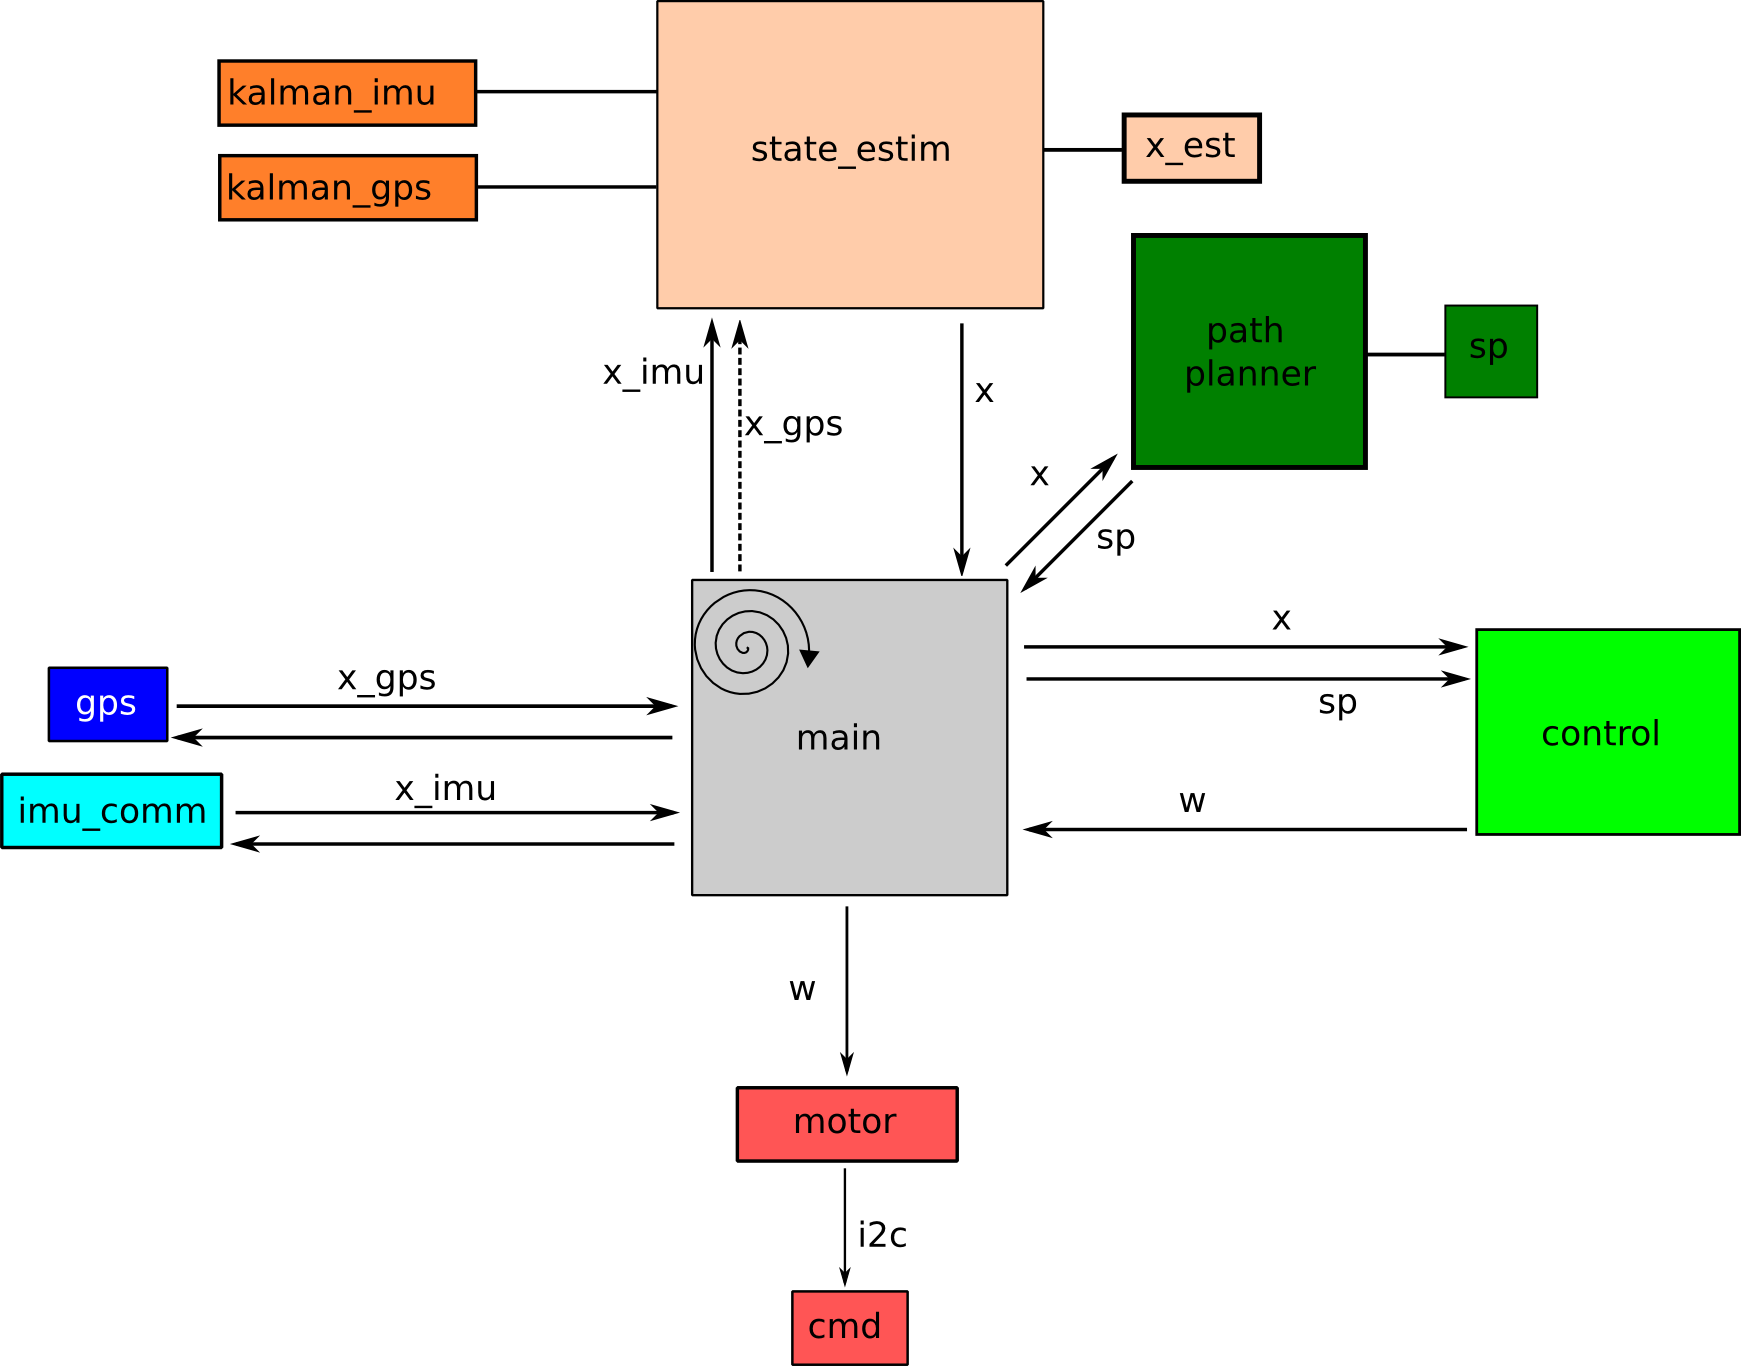
\includegraphics[width=0.5\textwidth]{./pics_codigo/code.png}
\caption{Estructura general del código.}
\vspace{-20pt}
\label{fig:codigo:code.png}
\end{wrapfigure}

El código tiene una estructura modular, está escrito en C, y cada bloque está implementado como una biblioteca. La estructura general del código se resume en la figura \ref{fig:codigo:code.png}.

\section{Inicializaci\'on}
\label{sec:software-init}

Para correr el programa principal (de ahora en más: \textit{main}) deber\'ia bastar con ejecutar el script \verb+src/go.sh+. Durante la inicializaci\'on el \textit{main} debe encontrar lo siguiente:\newline
\vspace{-20pt}

\begin{itemize}
\item \verb+imu_calib.txt+: Par\'ametros de calibraci\'on, la biblioteca \textit{imu\_comm} los necesita para convertir los datos crudos provenientes de la IMU.
\item \verb+K*.txt+: Matrices de control utilizados en el modo \textit{hover}.
\item \verb+lqr-*.txt+: Par\'ametros del algoritmo \textit{LQR}.
\item IMU: La IMU env\'ia datos a trav\'es de una \textit{UART} que es mapeada por el sistema operativo a un ``archivo'' \verb+/dev/tty*+. El \textit{main} recibe como par\'ametro la ruta a este archivo, o en su defecto un log \verb+imu_raw.txt+ generado por el \textit{main} en una ejecuci\'on previa.
\item GPS: Los datos provenientes del GPS  (\textit{USB}) son mapeados por el sistema operativo a \verb+/dev/ttyUSB*+. No se interactua directamente con este archivo, se utiliza la biblioteca \textit{gps\_comm} para iniciar un cliente que se comunique con el \textit{gpsd}, que es el programa que se encarga de leer y analizar los datos crudos provenientes del GPS. El \textit{gpsd} es iniciado por el script \verb+go.sh+.\newline
Si no se dispone de se\~nal del GPS se puede configurar un modo de prueba en el que se simulan los datos del GPS (a 1Hz) generando ceros, o números al azar dentro de un rango dado. Tambi\'en es posible deshabilitar completamente el GPS y trabajar con un vector de estados reducido. M\'as adelante se explica como configurar los distintos modos.
\item \verb+cmd+: El driver de los motores, encargado exclusivamente de env\'iar continuamente comandos \textit{i2c} a los ESCs con la \'ultima velocidad configurada\footnote{Los motores se apagan si no reciben comandos continuamente.}. La comunicaci\'on entre el driver y el \textit{main} se realiza mediante la biblioteca \textit{motor}, que a su vez se comunica con el driver mediante colas de kernel (IPC\footnote{\textit{Interprocess Communication}: \url{http://www.cs.cf.ac.uk/Dave/C}.}), utilizando la biblioteca \textit{uquad\_kernel\_msgq}.\newline
Durante pruebas, se puede configurar el driver para que simule la presencia de los motores, o para que lea de la entrada est\'andar. Ver \verb+src/i2c_beagle/README+ por informaci\'on sobre como compilar los distintos modos.
\end{itemize}

\section{Loop}
\label{sec:software-loop}

A continuaci\'on se describe un loop normal ejecutado por el \textit{main}, explicando brevemente las funcionalidades de cada una de las bibliotecas involucradas:
\begin{enumerate}

\item \textbf{imu:} La IMU genera datos nuevos cada 10ms. Al comienzo del loop, el \textit{main} revisa si hay datos nuevos, y en caso afirmativo llama a la biblioteca para que los lea. Cuando se completa una trama, los datos crudos se almacenan en una cola circular. Al terminar de recibir una trama, se vuelve al principio del loop para verificar que no hay m\'as nada para leer. En caso de haber m\'as datos entonces hay que leerlos para evitar atrasarse respecto a la IMU, en caso contrario se convierten los datos y se avanza.

\item \textbf{gps:} El GPS genera datos nuevos a una tasa mucho menor que la IMU. Cada vez que se dispone de una muestra nueva en la IMU, el \textit{main} revisa si tambi\'en hay un dato nuevo del GPS. Avanza aunque no se disponga de datos nuevos del GPS.

\item \textbf{kalman:} El filtro de Kalman est\'a implementado en la biblioteca \textit{kalman}. Recibe una estructura de datos generada por \textit{imu\_comm} y otra (opcional) generada por \textit{gps\_comm}. Mantiene una estructura de datos que almacena el estado estimado y las matrices de covarianza.

\item \textbf{path planner:} El m\'odulo generador de rutas est\'a implementado en la biblioteca \textit{path\_planner}. Compara el estado actual con el objetivo, y determina si se completó el objetivo actual\footnote{Solamente se implement\'o el modo \textit{hover}.}. En caso afirmativo, devuelve una bandera que le indicar\'a al m\'odulo de control que debe actualizar la matriz de control para ajustarla a la nueva trayectoria.

\item \textbf{control:} El m\'odulo de control est\'a implementado en la biblioteca \textit{control}. Mantiene una estructura con las matrices del control proporcional e integral (si corresponde). Recibe como argumento el estado estimado y la velocidad actual de los motores, y una estructura generada por \textit{path\_planner}, que indica el estado objetivo y la trayectoria a seguir. Devuelve la acci\'on de control a aplicar sobre los motores.

\item \textbf{motor:} Se env\'ia al driver una nueva velocidad deseada.

\end{enumerate}

Por información relativa a bloques, configuración, compilación, ejecución, etc, referirse a \verb+src/README+.

\section{M\'odulo \textit{imu\_comm}}
\label{sec:software:imu-comm}

A continuaci\'on se decriben algunas de las funcionalidades a destacar de la biblioteca \textit{imu\_comm}.

\begin{itemize}
\item \textbf{Calibración:} Se acumulan un conjunto de muestras que después se utilizan para estimar el offset de los giróscopos, la altura inicial, y pueden ser utilizados para inicializar el filtro de \textit{Kalman}. Durante la calibraci\'on es cr\'itico que el cuadric\'optero no se mueva, ya que en caso de hacerlo el offset de los gir\'oscopos ser\'a mal estimado.\newline
La inclinaci\'on durante la calibraci\'on afecta la estimaci\'on inicial del offset en los aceler\'ometros, pero en caso de no estar perfectamente horizontal se acomodar\'a luego de unos segundos, no es algo cr\'itico.
\item \textbf{Conversión:} Cargando parámetros de calibración, es posible convertir datos crudos provenientes de los sensores (cuentas de un ADC) a datos útiles:
  \begin{itemize}
  \item Aceler\'ometro $\rightarrow$ Aceleraciones.
  \item Gir\'oscopo $\rightarrow$ Velocidad angulares.
  \item Aceler\'ometro \verb~+~ Magnet\'ometro  $\rightarrow$ \'Angulos de Euler.
  \item Bar\'ometro $\rightarrow$ Altura y temperatura.
  \end{itemize}
Para la conversi\'on se utilizaron las calibraciones obtenida de la parte \ref{part:sensores-y-estimacion-del-estado}.
\begin{itemize}
\item Magnet\'ometro:
  \begin{equation}
    \label{eq:software:calib-lineal}
    conv = T.K_{inv}.(crudo - b)
  \end{equation}
  donde
  \begin{itemize}
  \item $T$ corrige el problema del \textit{cross axis sensitivity}.
  \item $K_{inv}$ es la inversa de la matriz de ganancias.
  \item $b$ Es un offset.
  \end{itemize}
\item Aceler\'ometro: Adem\'as de una calibraci\'on como la del magnet\'ometro, se implement\'o una compensaci\'on por temperatura:
  \begin{equation}
    \label{eq:software:acc}
    conv = T*inv(K)*(crudo - b + b_t*(t - t_0))    
  \end{equation}
  donde
  \begin{itemize}
  \item $T$, $K$ y $b$ cumplen el mismo rol que en el magnet\'ometro.
  \item $t$ es la temperatura actual, y $t_0$ la temperatura a la que se realiz\'o  la calibraci\'on de donde surgieron $T$, $K$ y $b$.
  \item $b_t$ es el factor que permite la compensaci\'on por temperatura.
  \end{itemize}
\item Gir\'oscopo: Se implement\'o algo an\'alogo a lo que se hizo para el acceler\'ometro, solo que al final se le resta un offset que se determina durante la calibraci\'on al inicio del programa. Esto es sencillo de estimar, ya que basta con que el cuadric\'optero no se mueva durante la calibraci\'on.\newline
Implementar algo an\'alogo pero para el caso del acceler\'ometro o del magnet\'ometro ser\'ia m\'as complicado, ya que requerir\'ia que el cuadric\'optero estuviese perfectamente horizontal o orientado hacia el norte, respectivamente.
\end{itemize}

\item \textbf{Verificaci\'on:} Se llevan 2 banderas que indican si la norma del vector de aceleraci\'on y la del vector de campo magn\'etico caen dentro del rango esperado. Esto puede ser de utilidad en el filtro de Kalman.

\item \textbf{Filtrado}: Se disponen de funciones que permiten obtener el elemento m\'as nuevo que a\'un no ha sido utilizado, o el resultado de aplicar un filtro FIR\footnote{Los coeficientes del filtro est\'an definidos en \textit{imu\_comm\_init()}.} a los 6 elementos m\'as recientes de la cola. Si por problemas de tiempo el \textit{main} se retrasa, pueden haber datos que nunca sean etiquetados como ``el dato m\'as nuevo'', ya que se leer\'a hasta ponerse al dia. De cualquier forma, ser\'an tomados en cuenta en el filtro.

\item \textbf{Modo \textit{FAKE}:} Seteando \verb+IMU_COMM_FAKE+ a 1, la biblioteca leerá de un log \verb+ascii+ en lugar de utilizar el puerto serie. En el modo \textit{FAKE} los tiempos no son un problema cr\'itico, ya que no correr\'a en tiempo real.
\end{itemize}

\section{M\'odulo \textit{kalman}}
\label{sec:software:kalman}

Aparte de implementar el filtro de Kalman descrito en la secci\'on \ref{chap:kalman}, la biblioteca \textit{kalman} se encarga de:


\begin{itemize}
\item Suavizar la estimaci\'on del \'angulo \textit{theta} dada por los aceler\'ometros y los magnet\'ometros. El ru\'ido presente en los aceler\'ometros, sumado a la mala performance del magnet\'ometro en lugares cerrados\footnote{Se prob\'o en lugares con muchos materiales met\'alicos, distorsionan las lecturas del magnet\'ometro.}, hace que sea necesario utilizar una l\'ogica de suavizado m\'as inteligente que un simple filtrado.
\item Llevar una estimaci\'on del \textit{bias} en los aceler\'ometros, cuyo objetivo es correjir errores sistem\'aticos.
\item Existe la posibildad de modificar la matriz de ruidos de observaci\'on, para las estimaciones realizadas a partir de informaci\'on proveniente del aceler\'ometro y del magnet\'ometro, en funci\'on de la norma del vector medido por cada sensor\footnote{Esta idea se tom\'o de \url{http://www.vectornav.com}.}.
\end{itemize}

Por detalles referirse a \verb+src/kalman/uquad_kalman.c+.

\section{M\'odulo de \textit{control}}
\label{sec:software:control}

La implementación del módulo de control se hizo en la biblioteca \textit{control}. Las funcionalidades implementadas son las siguientes:

\begin{itemize}
\item Control proporcional e integral.
\item Linealización del sistema en torno a una trayectoria y un \textit{set point} dados, y c\'alculo de las matrices de control correspondientes mediante \textit{LQR}.
\end{itemize}

Como se mencion\'o en \ref{sec:software:kalman}, el vector de estados almacenado por el filtro de Kalman incluye, adem\'as de las variables de estado del sistema, tres variables para la estimaci\'on del \textit{bias} de los aceler\'ometros. Estos tres t\'erminos no se utilizan en la m\'odulo de control.

\subsection{Control proporcional}
\label{sec:software:control-prop}


El control proporcional se rige por la siguiente ecuacion:
\begin{equation}
  \label{eq:software:prop}
  \vec{\omega}_{prop} = K_{prop} (\vec{sp}_x - \vec{x}_{est})
\end{equation}

donde
\begin{itemize}
\item $\vec{sp}_x$ Es el estado deseado, dado por el m\'odulo \textit{path\_planner}.
\item $\vec{x}_{est}$ Es la estimaci\'on del estado del sistema en el momento actual, dada por el filtro de Kalman.
\end{itemize}

\subsection{Control integral}
\label{sec:software:control-int}

El control integral es m\'as complejo, ya que incluye restricciones que son necesarias en la pr\'actica. A continuaci\'on se presenta un pseudoc\'odigo de la funci\'on que implementa la integral. Se aplica de manera independiente a cada una de las variables sobre la cual se desea llevar un control integral:
\begin{verbatim}
    integral = f_int(integral, err, Ts, th_dist, th_max, th_accum)

    // 1
    if (|err| > th_dist)
    {
      return integral;
    }

    // 2
    err = min(err * Ts, th_max);
    if (err < 0)
        err = max(err, -th_max);

    // 3
    integral = min(err + integral, th_accum);
    if(integral < 0)
        integral = max(integral,-th_accum);

    return integral;
\end{verbatim}

Los argumentos son:
\begin{itemize}
\item $err$: Diferencia entre el estado deseado y el actual: $err = sp_{x} - x$.
\item $integral$: Valor actual de la integral.
\item $Ts$: Per\'iodo de muestreo.
\item Umbrales (definidos, para cada una de las variables a integrar, en \newline\verb+src/control/control.h+) para los 3 controles implementados:
  \begin{enumerate}
  \item No se integra si la diferencia entre el estado actual y el deseado es mayor a un umbral dado por \verb+th_dist+, ya que se asume que esa situaci\'on debe ser resuelta por el control proporcional.
  \item Para evitar que la integral crezca muy r\'apido se utiliza un umbral \verb+th_max+, el m\'aximo error que se acepta integrar est\'a acotado por $th_{max}.Ts$.
  \item Por \'ultimo, si por alg\'un motivo la integral acumula demasiado el sistema tardar\'a mucho en recuperarse, por lo que se satura el integrador en \verb+th_accum+.
\end{enumerate}
\end{itemize}

Una vez calculada la integral, la ecuaci\'on que genera la acci\'on de control integral es:
\begin{equation}
  \label{eq:software:int}
  \vec{\omega}_{int} = K_{int} x_{int}
\end{equation}

\subsection{Control total}
\label{sec:software:control-total}

La acci\'on de control viene dada por
\begin{equation}
  \label{eq:software:control}
  \vec{\omega} = \vec{\omega}_{prop} + \vec{\omega}_{int}
\end{equation}

Las matrices de control para el modo \textit{hover} se encuentran en:
\begin{itemize}
\item Proporcional ($K_{prop}$): \verb+src/control/K_prop_pptz.txt+
\item Integral ($K_{int}$): \verb+src/control/K_int_full_pptz.txt+.
\end{itemize}

Estas matrices son utilizadas en el modo \textit{hover}, donde no hace falta utilizar \textit{LQR}. Son archivos de texto plano, y si se modifican entonces los cambios ser\'an tomados en cuenta al ejecutar el script \verb+src/go.sh+.

\section{Generador de rutas}
\label{sec:software:generador-de-rutas}

La versi\'on actual del c\'odigo implementa solamente el modo \textit{hover}. El \textit{set point} inicial cero para todas las variables, excepto para el \'angulo $\theta$, para el cual se tomar\'a el \'angulo inicial, y para la altura (1m por defecto).

Se pueden modificar las condiciones de \textit{hovering} en \verb+src/main/main.c+.

En \textit{MatLab} hay una implementaci\'on del generador de rutas, queda pendiente pasarlo a \verb+C+.

\subsection{Modo Manual}
\label{sec:software:modo-manual}

En el modo \textit{hover} es posible modificar el \textit{set point} desde la li\'nea de manera remota. Para ellos, iniciar el \textit{main} y apretar la tecla \verb+m+, seguida de un \verb+ENTER+. Esto setear\'a el \textit{main} en modo manual, y estar\'a dispuesto a recibir comandos. Cada comando modificar\'a el \textit{set point}, y ser\'a considerado solamente luego de presionar \verb+ENTER+. La lista de comandos se encuentra en \verb+src/common/manual_mode.h+.

\section{Driver de los motores y m\'odulo \textit{motor}}
\label{sec:software:cmd-motor}

La biblioteca \textit{motor} y el driver \verb+src/i2c_beagle/cmd_motores.c+ (de ahora en m\'as \textit{cmd}) tienen una fuerte relaci\'on, y deben ser coherentes. El driver no se pudo incluir como una biblioteca m\'as, ya que requiere de un encabezado que solamente est\'a disponible en la \textit{BeagleBoard}.

Algunas consideraciones relevantes:
\begin{itemize}
\item El \textit{cmd} espera una velocidad superior a cierto m\'inimo, de lo contrario no arrancar\'a los motores. Este umbral debe estar apareado, de los contrario \textit{motor} ser\'a incapaz de arrancar los motores en el momento apropiado.\newline
Luego del arranque, \textit{motor} se encargar\'a de no enviar valores por debajo de los valores definidos como m\'inimo y m\'aximo. Usar valores por debajo del m\'inimo puede hacer que se apaguen los motores, y valores por encima del m\'aximo pueden sobrecalentar los contactos de los cables que alimentan a los motores. El m\'aximo tambi\'en debe estar apareado entre el \textit{cmd} y \textit{motor}.\newline
El \textit{cmd} reportar\'a un error en caso de recibir valores fuera de rango.

\item Al arrancar los motores, el \textit{cmd} setea velocidades en torno una rampa\footnote{La implementaci\'on son valores que saltan por encima y por debajo de la rampa, esta t\'ecnica ha demostrado ser eficiente para hacer arrancar los motores.} desde 0 hasta el valor definido como m\'inimo, al cual el cuadric\'optero no es capaz de levantar vuelo.

\item Por cada comando que \textit{motor} env\'ia al \textit{cmd}, este \'ultimo responde con un \textit{ack}. Así \textit{motor} verifica que el \textit{cmd} est\'a funcionando\footnote{Solamente se verifica que hay comunicaci\'on, pero la implementaci\'on es tal que si la comunicaci\'on es exitosa, entonces todo deber\'ia estar funcionando correctamente.}.

\end{itemize}

\textbf{ADVERTENCIA:} Cualquier mensaje de error reportado por el \textit{cmd} es motivo suficiente para detener el vuelo y analizar el problema.

\section{Tiempos}
\label{sec:software:tiempos}

El per\'iodo de muestreo resulta fundamental para tanto el filtro de Kalman como el control integral. Para llevar el tiempo se dispone de funciones del sistema operativo que tienen precisi\'on de microsegundos. Se consulta el tiempo al momento de llamar a las bibliotecas \textit{kalman} y \textit{control} y se lo almacena, de manera de poder estimar un per\'iodo de muestreo a partir del tiempo transcurrido entre llamadas sucesivas.

El m\'aximo retardo entre que se lee un dato nuevo de la IMU y que se efectua una acci\'on de control es de 10ms, en general es de 8ms. Retardos mayores llevar\'ian a perder muestras de la IMU, lo cual ser\'ia detectable en el log de errores. Por m\'as informaci\'on sobre los logs referirse al anexo \ref{chap:anexo-codigo}.

\section{Comunicaci\'on}
\label{sec:software-comm}

La comunicaci\'on con la \textit{BeagleBoard} se hace mediante \textit{ssh}. En el anexo \ref{chap:anexo-codigo} se explica como configurar las partes involucradas.

\section{Configuraci\'on}
\label{sec:software-config}

\subsection{Parametros del sistema}
\label{sec:software:param-del-sistema}

\begin{itemize}
\item \verb+src/common/uquad_types.h+: La mayor parte de los par\'ametros del sistema est\'an definidos aqui, entre ellos la masa, el tensor de inercia, el orden del vector de estados, per\'iodo de muestreo, etc.

\item \verb+src/CMakelists.tx+: La variable \verb+USE_GPS+ es un booleano que determina si ha de utilizarse el GPS o no.

\item \verb+src/common/uquad_config.h+: En este archivo se configura el modo de funcionamiento. Se realizan controles sobre la opciones elegidas, evitando que el usuario seleccione un modo inv\'alido. Es posible elegir:
  \begin{itemize}
  \item Trabajar con 8 estados o con 12.
  \item Guardar logs.
  \item Habilitar control integral.
  \item Si el GPS fue habilitado, es posible utilizar un GPS de mentira, \'util para pruebas.
  \item Cada cuantas muestras de la IMU se desea efectuar una acci\'on de control.
  \end{itemize}

\item \verb+src/imu/imu_comm.h+: Permite:
  \begin{itemize}
  \item Permite configurar el largo del filtro LPF, cuyos coeficientes se definen en \verb+src/imu/imu_comm.c+.
  \item Elegir entre leer de un log o de la IMU.
  \item Elegir el largo de la cola circular donde se almacenan los datos crudos (debe ser mayor que la cantidad de coeficientes del filtro).
  \item Seleccionar cuantas muestras han de usarse para la calibraci\'on (512 por defecto).
  \end{itemize}
\end{itemize}

\subsection{Control}
\label{sec:software:config-control}

Para el modo \textit{hover}, basta con modificar las matrices en \verb+src/control/+, de donde se leen las ganancias a utilizar. Para el resto de los modos hay que modificar los archivos de donde se configura el \textit{LQR}. En la secci\'on \ref{sec:software:param-del-sistema} se explic\'o como modificar la estrateg\'ia de control.

\subsection{Ruidos Kalman}
\label{sec:software:config-kalman}

En \verb+src/kalman/uquad_kalman.c+ se definen los ruidos de transici\'on de estados y de observaci\'on. Los valores que var\'ian al utilizar el modo de covarianza din\'amica (en funci\'on de la norma de los vectores de aceleraci\'on y campo magn\'etico) se definen en \verb+src/kalman/uquad_kalman.h+.

\end{document}